\chapter{Experiments and Results}\label{ch:results}

\section{Experiments}
Simulations were developed using Matlab and Simulink.\\

%ADD chosen parameters GC


\subsection{LQR Control}

***************************************\\
Benchmark can be a simple control design \\
Benchmark can be Praveen's MPC controller to compare results \\
Benchmark can be open loop response Figure \ref{fig:QROL}.\\
\begin{figure}[h!]
	\centering
	\makebox[\textwidth][c]{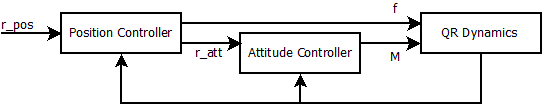
\includegraphics[width=.2\paperwidth]{./StyleStuff/QRloop.png}}
	\caption{Open Loop control QR \label{fig:QROL}}
\end{figure}

***************************************\\

Benchmark can be an \a{LQR} controller, \ref{app:model}
\begin{figure}[h!]
	\centering
	\makebox[\textwidth][c]{\includegraphics[width=.45\textwidth]{./StyleStuff/dcsc.png}}
	\caption{LQR control design\label{fig:}}
\end{figure}		

%ADD chosen parameters LQR



\subsection{Performance Criteria}
***************************************\\
Performance that can be evaluated for the cases in Figure \ref{fig:routes}. Performance can be specified as the following items.
\begin{outline}
	\1 Step Response
	\2 Settling time (if swing minimization is important)
	\2 Rising time (important if time critical)
	\2 Overshoot (if max swing is critical)
	\2 Steady state error / swing of load (if accuracy is important)
	
	\1 Disturbance Rejection
	
	\1 Trajectory tracking
	\2 Can we minimize time, while minimizing position error (All Cases)
	\2 Minimum position error (All Cases)
	\2 Maximum amplitude/frequency of wave with respect to stability (Case B)
	
	\1 Computational Effort (?)
\end{outline}

Explain cases, why interesting and what can be expected?\\

\subsection{Case A}
\subsection{Case B}
\subsection{Case C}

\begin{figure}[h!]
	\centering
	\makebox[\textwidth][c]{\includegraphics[width=.2\paperwidth]{./StyleStuff/dcsc.png}}
	\caption{Cases of which the performance could be evaluated \label{fig:routes}}
\end{figure}

\section{Command Filtering}
%ADD Why is Command Filtering needed? 
Consequence of backstepping control is that inner control loops depend on the the output of outer control loops. The controllers are functions of these generated outputs and their derivatives. This can be calculated analytically, which can be tedious or by estimating with the use of a Command Filter as explained by \cite{Djapic} 
%CHECK Djapic of andere?

A command filter is implemented to compute $ \dot{R}_c, \ddot{R}_c,\dot{q}_c, \ddot{q}_c $, the virtual control command to stabilize the loop within. \cite{Farrell2009}

Examples from \cite{Farrell2008} and \cite{Djapic2008}. 

***************************************\\
%ADD Pro Con Command filter
Easy implementation. Less computational effort.

Less accurate, because filters high frequency signals.

***************************************\\

The load attitude controller generates a commanded QR attitude $ R_c $ and its derivative $ \dot{R}_c $. In the same fashion, the load position controller generates a commanded load attitude $ q_c $ and its derivative $ \dot{q}_c $. The controllers are functions of these commanded signals and their derivatives. Instead of analytic differentiation of these signals, they are obtained by integration by applying a third order low pass filter to the original signals $ R_c^o $ and $ q_c^o $. The transfer function of the original commanded input signal $ X_c^o $ and the filtered output $ X_c $ has the form
\begin{equation}\label{key}
\frac{X_c(s)}{X_c^o(s)}=H(s)=\frac{\omega_{n1}}{s+\omega_{n1}}\cdot\frac{\omega_{n2}^2}{s^2+2\zeta\omega_{n2}s+\omega_{n2}^2}
\end{equation}
Where $ x_c $ is the filtered signal, $ \zeta $ the damping ratio and $ \omega_n $ the undamped natural frequency. See Figure \ref{fig:CF}.
The state space implementation of this third order filter is \cite{Djapic2008}
%CHECK waar dit ook alweer vandaan kwam. Reference in Djapic/Farell -> 3e order voor bacterieen ofzo
\begin{align}\label{key}
\dot{x}_1 &= x_2\\ %dxc
\dot{x}_2 &= x_3\\ %ddxc
\dot{x}_3 &= -(2\zeta \omega_{n2}+\omega_{n1})x_3-(2\zeta\omega_{n1}\omega_{n2}+\omega_{n2}^2)x_2-(\omega_{n1}\omega_{n2}^2)(x_1-x_c^o)
\end{align}
where $ x_1 = x_c$, $ x_2 = \dot{x}_c$ and $ x_3 = \ddot{x}_c$. 

\begin{figure}[h!]
	\centering
	\makebox[\textwidth][c]{\includegraphics[width=.45\textwidth]{./StyleStuff/dcsc.png}}
	\caption{Representation of the command filter\label{fig:CF}}
\end{figure}		

\begin{align}\label{eq:CF}
\frac{x_c}{x_c^o}&=\frac{\omega_{n1}}{s+\omega_{n1}}\cdot\frac{\omega_{n2}^2}{s^2+2\zeta\omega_{n2}s+\omega_{n2}^2}\\
\Rightarrow x_c^{'''}&=-(2\zeta\omega_{n2}+\omega_{n1})x_c^{''}-(2\zeta\omega_{n1}\omega_{n2}+\omega_{n2}^2)x_c^{'}-(\omega_{n1}\omega_{n2} ^2)(x_c-x_c^o)
\end{align}

\section{Results}
\subsection{Case A}
\subsection{Case B}
\subsection{Case C}


\section{Conclusion}

